\documentclass[11pt,a4paper]{article}
\usepackage[utf8]{inputenc}
\usepackage{amsmath}
\usepackage{amsfonts}
\usepackage{easy-todo}
\usepackage{amssymb}
\usepackage{graphicx}
\usepackage[left=2cm,right=2cm,top=2cm,bottom=2cm]{geometry}
\usepackage[colorlinks,linkcolor=black,citecolor=black,filecolor=black]{hyperref}
\usepackage{listings}
\catcode`^=\active
\def^#1^{\texttt{#1}}


\begin{document}
\title{Autonomous Agents - Assignment 1}
\author{BasVeeling (10767770) \\ \and Sebastian Droeppelmann (?) \\ \and Fritjof Buettner (10876782)}
\maketitle
\listoftodos
\section{Introduction}
\subsection{Project structure}
We decided to model the predator/prey problem in Python. We chose an object-oriented structure to make the code reusable and minimize repetitions. In order to assure correct functionality of the algorithms at a fine-grained level, we make use of Python's unit-test framework.
\begin{figure}[h!]
  \caption{Class diagram}
  \centering
    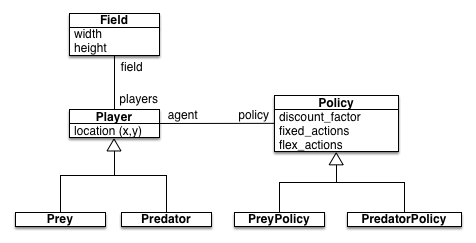
\includegraphics[width=0.6\textwidth]{classdiagram}
   \label{fig:classdiagram}
\end{figure}

The file \texttt{main.py} in the root directory of the project executes all the tasks required in the assignment and prints the according output to the console. The models for field, players and their respective policies are located in the subdirectory \texttt{models}. Their relationship is illustrated in figure~\ref{fig:classdiagram}. Both \texttt{Predator} and \texttt{Prey} class are children of the \texttt{Player} superclass, which provides common attributes such as the location and policy fields. 

There is a bidirectional connection between the field and the players on it, such that the field maintains a list of active players, who in return hold a reference to the field they are on in order to receive sensory information like the position of other players. Every player has their own policy (even the prey, which is not an agent at this point).
Furthermore, the field also provides the function \texttt{is\_ended()} which can be used to check whether the predator has caught the prey.

For a more human-readable output, the field implements the function \texttt{print\_field()} which prints an ASCII-graphical representation of the field to the console, with a \textbf{\texttt{X}} denoting the position of the predator(s) and a \textbf{\texttt{O}} denoting the position of the prey(s).

\section{Question 1: Environment Simulator}
We implemented the simulator as described above. The ^main.py^ ^as011()^ function runs one simulation with a random policy for both the prey and the predator. It initializes a 11x11 field with one predator and one prey. For every time step the predator performance an action based on its policy (^predator.act()^), and this will update the field, until the game is over (^field.is\_ended()^).

The ^main^ functions calls this simulation 100 times and calculates the average and stdev of the running time, this results in:
\begin{lstlisting}[language=bash]
$ python main.py
Mean runtime: 0.01544s (standard deviation: 0.0133)
Mean number of iterations: 1026.88 (standard deviation: 888.41)
\end{lstlisting}

\subsection{Random Policy}
\todo{Explain the random policy here as soon as we have nailed it down}
\section{Question 4: Value Iteration}
\todo{Write a section about value iteration}

\todo{Test for convergence speed (in number of iterations), for different discount factors: at least 0.1, 0.5, 0.7 and 0.9, and report on the results.}
\section{Conclusion}
It's all great.
\end{document}